\documentclass{article}

\usepackage[final]{neurips_2023}

\usepackage[utf8]{inputenc}
\usepackage[T1]{fontenc}
\usepackage{hyperref}
\usepackage{url}
\usepackage{booktabs}
\usepackage{amsfonts}
\usepackage{amsmath}
\usepackage{nicefrac}
\usepackage{microtype}
\usepackage{xcolor}
\usepackage{graphicx}

% Draft-status notes (remove before submission)
\newcommand{\draftnote}[1]{\textcolor{red}{\textbf{[DRAFT NOTE: #1]}}}

\title{Measuring the Tightness Gap: An Empirical Audit of\\Differential Privacy Guarantees in DP-SGD}

\author{%
  Mohamad Faour \\
  Department of Electrical and Computer Engineering\\
  EECE 608 --- Final Project\\
  \texttt{msf20@mail.aub.edu} \\
}

\begin{document}

\maketitle

\begin{abstract}
Differential privacy (DP) provides formal guarantees that bound the privacy leakage of a trained model, yet these guarantees are derived under worst-case assumptions that need not match the leakage demonstrated by a concrete auditing attack. This paper treats privacy auditing as a framework problem: to compare theory and empirical evidence reliably, the implementation must keep threat models separate, compute theoretical and empirical quantities consistently, preserve reproducibility across seeds, and reject statistically unsupported leakage claims. We build an end-to-end DP-SGD auditing framework with two tracks: evaluator-controlled canary insertion and passive final-model-only membership inference. On MNIST, the framework reproduces the expected qualitative distinction between threat models while conservative Wilson confidence bounds prevent small-sample artifacts from being reported as privacy violations. The main contribution is therefore not a new attack, but a validated experimental scaffold for measuring the tightness gap between $\varepsilon_{\text{upper}}$ from DP accounting and $\varepsilon_{\text{lower}}$ from concrete audits. We document the validation process, including seed propagation failures, score-direction errors, sparse-tail pathologies, and a GDP-based estimator that is useful diagnostically but invalid as a lower bound when it exceeds the theoretical upper bound.
\end{abstract}

\section{Introduction}

Differential privacy (DP) provides a formal stability guarantee for randomized algorithms. A randomized mechanism $\mathcal{M}$ satisfies $(\varepsilon,\delta)$-DP if, for all neighboring datasets $D$ and $D'$ that differ in one record and for all measurable output events $S$,
\begin{equation}
    \Pr[\mathcal{M}(D) \in S] \leq e^\varepsilon \Pr[\mathcal{M}(D') \in S] + \delta .
\end{equation}
In this definition, $\varepsilon$ controls the multiplicative privacy-loss bound and $\delta$ allows a small probability of failure~\citep{dwork2014algorithmic}. DP-SGD operationalizes this guarantee for neural network training by clipping per-example gradients and adding Gaussian noise at each optimization step~\citep{abadi2016deep}. A privacy accountant then returns an upper bound, denoted $\varepsilon_{\text{upper}}$, for a fixed value of $\delta$.

However, the accountant-derived $\varepsilon_{\text{upper}}$ is a worst-case upper bound over neighboring datasets and adversarial observations. For a fixed trained model and a concrete auditing procedure, the empirically demonstrable privacy leakage may be much smaller. This paper studies the resulting \emph{tightness gap}: the distance between the theoretical privacy upper bound and the empirical lower bound supported by an audit.

Understanding this gap matters for two reasons. First, a large gap may indicate that the deployed mechanism pays a substantial utility cost for a worst-case guarantee that is loose for the evaluated setting. Second, the same gap may also indicate that the available auditors are weak. A careful audit framework must therefore distinguish loose accounting from insufficient attack strength.

Recent work has begun to close this gap. Nasr et al.~\citep{nasr2023tight} showed that carefully designed auditing schemes can produce nearly tight privacy estimates with just two training runs. Steinke et al.~\citep{steinke2023privacy} pushed this further, obtaining tight audits from a single run by inserting multiple canaries at once. On the passive side, membership inference attacks~\citep{shokri2017membership, carlini2022membership} provide a natural way to probe leakage when the auditor can only observe the final model.

This paper asks: how close are empirical auditing lower bounds to the theoretical privacy upper bounds reported by DP accountants under DP-SGD? We answer this question by building a reproducible framework rather than a new auditing algorithm. The framework brings together DP-SGD training, RDP and PLD accounting, active canary auditing, passive membership inference, confidence-aware lower-bound estimation, artifact validation, and sanity checks in one workflow. Its purpose is to identify which leakage claims remain credible after changing seeds, increasing the audit budget, checking score direction, and rejecting estimates that contradict the theoretical privacy contract.

\section{Related Work}

The theoretical foundations of differential privacy are laid out in the monograph by Dwork and Roth~\citep{dwork2014algorithmic}. DP-SGD~\citep{abadi2016deep} made it practical to train neural networks with DP guarantees, and R\'{e}nyi DP~\citep{mironov2017renyi} tightened the accounting. Opacus~\citep{yousefpour2021opacus} provides the PyTorch implementation used in this study.

On the auditing side, membership inference~\citep{shokri2017membership} established the core paradigm, and Carlini et al.~\citep{carlini2022membership} refined it with principled likelihood-ratio attacks. Jagielski et al.~\citep{jagielski2020auditing} introduced auditing-by-poisoning for DP-SGD, and Nasr et al.~\citep{nasr2021adversary} instantiated a ladder of progressively stronger adversaries on the same training setup, establishing that the audit gap shrinks as adversary capabilities approach the assumptions of the accounting proof. Nasr et al.~\citep{nasr2023tight} subsequently achieved tight audits with two runs---demonstrating along the way that part of the theory--practice gap is an accounting artifact, since empirical leakage matches tighter f-DP-style accounting while RDP-reported $\varepsilon$ is loose---and Steinke et al.~\citep{steinke2023privacy} reduced the requirement to one run. Annamalai and De Cristofaro~\citep{annamalai2024nearly} attribute much of the remaining black-box gap to average-case initialization, and report that the gap varies with the noise multiplier and number of steps. PANORAMIA~\citep{kazmi2024panoramia} proposed passive auditing without retraining using synthetic non-members. Lu et al.~\citep{lu2022general} present a general auditing framework centered on stronger poisoning attacks and improved hypothesis-testing machinery; our contribution differs in that we do not strengthen attacks but attribute the measured gap across its sources on shared runs.

On the estimation side, a line of work treats event and threshold selection as the central validity obstacle in converting attack outcomes to $\varepsilon$ lower bounds: Bayesian credible intervals~\citep{zanella2023bayesian}, non-parametric f-DP trade-off estimation~\citep{askin2025fdp}, and density-estimation audits~\citep{koskela2025density}. Concurrently with this work, Michel et al.~\citep{michel2026sequential} prove coverage for a calibration/evaluation sample-split estimator closely related to the holdout construction we deploy (Section~\ref{sec:validity}). Cebere et al.~\citep{cebere2026zerorun} formalize the distribution-shift confound in observational audits: an attack can appear to succeed by exploiting feature differences between member and non-member populations rather than algorithmic leakage. Fundamental limits on one-run auditing~\citep{keinan2025onerun} and on the sample complexity of membership inference~\citep{haghifam2025sample} constrain what any fixed auditor family can certify. The recent SoK by Annamalai et al.~\citep{annamalai2026sok} systematizes DP auditing along threat-model, attack, and evaluation-function axes and poses gap attribution as an open problem; we adopt their vocabulary throughout.

We do not propose a new auditing algorithm. Prior work established each gap source in isolation---accounting~\citep{nasr2023tight}, threat model~\citep{nasr2021adversary,annamalai2024nearly}, and statistical estimation~\citep{zanella2023bayesian,askin2025fdp,koskela2025density}. Our aim is a controlled quantification of these shares on the \emph{same} training runs, in a reproducible pipeline with confidence-aware reporting, artifact validation, and sanity checks built in.

\section{Preliminaries and Definitions}
\label{sec:preliminaries}

We fix definitions precisely, because several quantities that circulate informally in the auditing literature (``empirical epsilon,'' ``tightness,'' ``the gap'') acquire different meanings under different adjacency relations, accountants, and estimators. Throughout, our vocabulary for threat models follows the systematization of Annamalai et al.~\citep{annamalai2026sok}.

\textbf{Adjacency.} Two datasets $D, D'$ are \emph{add/remove adjacent} if one is obtained from the other by adding or removing exactly one record. All guarantees and audits in this paper use add/remove adjacency, matching the convention under which Opacus and the \texttt{dp\_accounting} library analyze DP-SGD. This choice is load-bearing for auditing: the audit game must insert or withhold a record, not substitute one, or the demonstrated leakage is measured against a different (replace-one) definition with a different theoretical bound.

\textbf{Mechanism and accountants.} DP-SGD with clipping norm $C$, noise multiplier $\sigma$, Poisson sampling rate $q$, and $T$ steps is a fixed randomized mechanism $\mathcal{M}$. A \emph{privacy accountant} $A$ maps $(\sigma, q, T, \delta)$ to a certified bound $\varepsilon^{A}_{\text{upper}}$ such that $\mathcal{M}$ is $(\varepsilon^{A}_{\text{upper}}, \delta)$-DP. Accountants differ in tightness for the \emph{same} mechanism: we compute both $\varepsilon^{\text{RDP}}_{\text{upper}}$ (R\'{e}nyi DP composition~\citep{mironov2017renyi}) and $\varepsilon^{\text{PLD}}_{\text{upper}}$ (privacy loss distribution accounting, computed with \texttt{dp\_accounting}; never an analytical approximation). Since both are valid upper bounds on the same privacy loss, $\varepsilon^{\text{PLD}}_{\text{upper}} \le \varepsilon^{\text{RDP}}_{\text{upper}}$ in our regime, and the difference is pure accounting looseness.

\textbf{The audit game and empirical lower bounds.} An audit instantiates the hypothesis-testing interpretation of DP~\citep{balle2020hypothesis}: a challenger trains with or without a target record (under the add/remove game, with membership decided by an independent fair coin per record), and the auditor guesses membership from its observations. Any auditor achieving true positive rate $\mathrm{TPR}$ and false positive rate $\mathrm{FPR}$ at some decision threshold witnesses
\begin{equation}
    \varepsilon_{\text{lower}} \;=\; \ln\!\frac{\mathrm{TPR} - \delta}{\mathrm{FPR}},
\end{equation}
provided $\mathrm{TPR} > \mathrm{FPR}$~\citep{jagielski2020auditing}. Because rates are estimated from finite samples, a \emph{statistically valid} lower bound must hold with stated confidence over the audit's randomness; we call an estimator \emph{selection-valid} if its confidence guarantee survives the choice of the reported threshold (Section~\ref{sec:validity} shows the standard sweep is not, and how we repair it). $\varepsilon_{\text{lower}}$ is always attack-and-estimator relative; it lower-bounds what \emph{this} auditor with \emph{this} estimator certifies, not the mechanism's true leakage.

\textbf{Tightness and the gap.} For a fixed training run, accountant $A$, threat model $\theta$, and estimator $E$:
\begin{equation}
    \Delta\varepsilon(A, \theta, E) = \varepsilon^{A}_{\text{upper}} - \varepsilon^{\theta,E}_{\text{lower}},
    \qquad
    \rho(A, \theta, E) = \varepsilon^{\theta,E}_{\text{lower}} / \varepsilon^{A}_{\text{upper}}.
\end{equation}
If $\rho = 1$ the auditor has matched the certified bound; $\rho \ll 1$ means the bound is loose \emph{or} the auditor or estimator is weak --- the ambiguity this paper is designed to resolve.

\textbf{Gap decomposition.} Holding the training runs fixed and toggling one factor at a time yields attributable shares: the \emph{accounting share} is the fraction of $\Delta\varepsilon(\text{RDP}, \theta, E)$ removed by switching to PLD accounting alone; the \emph{estimator share} is the further fraction removed by switching estimators at fixed $(A,\theta)$; the \emph{threat-model share} is the change from passive to evaluator-controlled auditing at fixed $(A,E)$. The residual is attributed only under the saturation condition below.

\textbf{Saturation criterion.} Let $\varepsilon_{\text{lower}}(K)$ denote the certified bound as auditor strength grows (for LiRA-style attacks, $K$ is the number of shadow models). We say the auditor family has \emph{saturated} when $\varepsilon_{\text{lower}}(K)$ stops improving over a doubling ladder of $K$ within confidence bounds. Saturation is a \emph{necessary condition} for attributing the residual gap beyond the auditor family: while $\varepsilon_{\text{lower}}(K)$ still climbs, attribution is premature. It is not sufficient --- plateaus are attack-family-specific, and matching the optimal adversary can require infeasible reference information~\citep{haghifam2025sample, keinan2025onerun} --- so a plateau licenses only the statement ``the residual is not recoverable by this family at this budget.''

\textbf{Per-$\varepsilon$ hyperparameter optimization.} Comparisons across privacy levels are confounded if a single hyperparameter setting is reused at every $\varepsilon$ (models at some noise levels would be under-trained, mixing optimization failure into the measured gap). For each target $\varepsilon$ in our sweep we therefore tune $(\text{learning rate}, \text{batch size}, \text{epochs}, C)$ with Optuna~\citep{akiba2019optuna}, re-solving $\sigma$ for every trial so that $\varepsilon^{\text{PLD}}_{\text{upper}}$ is held exactly at the target while utility is maximized; audited models are then retrained from scratch with the winning configuration under the canonical seeds. Following standard practice, the tuning phase is treated as out-of-band for the audited guarantee~\citep{papernot2022hyperparameter}; we state this explicitly because hyperparameter choice itself measurably changes empirical leakage at fixed $(\varepsilon,\delta)$~\citep{hu2025empirical}, which is an argument for --- not against --- auditing the tuned configuration actually deployed.

\subsection{Two Threat Models}

We keep two experiment tracks completely separate in code, configuration, and outputs:

\textbf{Track 1 -- Canary stress testing.} The evaluator modifies the training data by inserting crafted ``canary'' examples before DP-SGD training. After training, the evaluator distinguishes inserted canaries from held-out control canaries. This is the stronger threat model because the evaluator controls part of the training distribution; it should be interpreted as a controlled stress test.

\textbf{Track 2 -- Passive auditing.} The auditor observes only the released model and cannot modify the training data. The auditor queries the model on candidate member and non-member examples and separates them using output-derived scores. This weaker threat model is closer to post-deployment auditing, where the auditor has access to the final model and a candidate evaluation set.

\section{Methodology}

\subsection{Model and Training}

We use MNIST~\citep{lecun1998mnist} with a small two-layer MLP: the $28 \times 28$ images are flattened and passed through a $784 \to 64$ linear layer with ReLU, then a $64 \to 10$ output layer. We train with DP-SGD using the Opacus library~\citep{yousefpour2021opacus} with batch size 256, gradient clipping norm $C = 1.0$, noise multiplier $\sigma = 1.1$, learning rate 0.15, and $\delta = 10^{-5}$, for a single epoch on the full 60{,}000-example training set. Under these settings, the R\'{e}nyi DP accountant~\citep{mironov2017renyi} in Opacus reports $\varepsilon_{\text{upper}} = 0.771$.

Each experiment is repeated across three random seeds (123, 124, 125). Reproducibility artifacts and schema validation are described in Section~\ref{sec:reproducibility}.

\subsection{Canary Stress Testing}

The canary pipeline works in five steps. First, we \textbf{generate} canary images by placing structured pixel patches at deterministic positions within a blank $28 \times 28$ image, assigned a target label. We currently have three strategies of increasing aggressiveness: \texttt{random\_canaries} (3-pixel patches at intensity 0.8), \texttt{improved\_canaries} (4-pixel patches at 0.95), and \texttt{optimized\_canaries} (5-pixel patches at full intensity). Second, we \textbf{insert} 32 canaries into the training set at an insertion rate of 0.5\%. Third, we \textbf{retrain} a fresh DP-SGD model on the augmented data with the same hyperparameters. Fourth, we \textbf{score} inserted canaries against held-out decoys by computing the target margin---the gap between the target-label logit and the strongest non-target logit---on each. Fifth, we \textbf{repeat} the process across two audit seeds per training seed to accumulate a distribution of membership scores.

\subsection{Passive Membership Inference}

The passive pipeline loads a trained checkpoint and constructs a balanced query set: half known training members, half known non-members (held-out test examples). We tried four different scoring rules to see which gives the strongest signal:

\begin{itemize}
    \item \emph{Probability margin} (labeled \texttt{logit\_margin} in code): the gap between the top two softmax probabilities, $s(x) = p_1 - p_2$ where $p_1 \geq p_2 \geq \cdots$ are the sorted softmax outputs.
    \item \emph{Max probability}: the maximum softmax probability.
    \item \emph{Negative loss}: the negative of the cross-entropy loss on the true label.
    \item \emph{Score fusion}: a combination of the above using percentile rank normalization.
\end{itemize}

The baseline query budget is 128 examples (64 members, 64 non-members). We also experimented with temperature scaling calibration using 20\% of the query budget as a held-out calibration set.

\subsection{Estimating the Empirical Lower Bound}

Given the member and non-member score distributions from either auditing track, we estimate $\varepsilon_{\text{lower}}$ as follows. We sweep over all unique score values as thresholds. At each threshold $\tau$, we compute the true positive rate $\text{TPR}(\tau)$ and false positive rate $\text{FPR}(\tau)$, then convert to a privacy loss estimate:
\begin{equation}
    \hat{\varepsilon}(\tau) = \max\!\left(0, \;\ln\!\left(\frac{\text{TPR}(\tau) - \delta}{\text{FPR}(\tau)}\right)\right)
\end{equation}
We pick the threshold that maximizes $\hat{\varepsilon}$, subject to a member-favoring constraint ($\text{TPR} > \text{FPR}$). To avoid overstating leakage due to small-sample noise, we compute Wilson score intervals~\citep{wilson1927probable} for both rates and report a conservative bound using the lower CI for TPR and upper CI for FPR. When the best threshold falls in a sparse tail (fewer than 5 observations or under 12.5\% of samples), we flag it and default to the conservative bound.

\textbf{Selection-valid holdout estimation.} Maximizing $\hat{\varepsilon}$ over all candidate thresholds and then reporting a confidence bound computed on the \emph{same} sample voids the interval's nominal coverage: the maximum over thousands of dependent candidates is anti-conservative by construction. In null-coverage simulations with pure-noise scores, the in-sample path reports spuriously positive ``conservative'' bounds (up to $\varepsilon = 0.43$), and in-sample \emph{point} estimates under the null range from $0.59$ to $3.16$ across shadow-model counts---direct evidence that point estimates at these budgets must never be quoted. Our final reporting path therefore uses a deterministic sample split: the threshold is selected on one half of the scores and the Wilson bound is certified at that single fixed threshold on the other half, restoring valid coverage ($\varepsilon = 0$ in 200/200 pure-noise repetitions). A closely related calibration/evaluation split, with a coverage proof and a DKW-envelope alternative that avoids splitting, appears concurrently in Michel et al.~\citep{michel2026sequential}; our contribution on this axis is the empirical demonstration of the violation's magnitude in standard DP-SGD audit pipelines.

We also implemented a GDP-inspired AUC estimator as a diagnostic check, motivated by Gaussian differential privacy~\citep{dong2019gaussian} and hypothesis-testing interpretations of privacy~\citep{balle2020hypothesis}. This estimator maps the empirical AUC between member and non-member scores to a Gaussian DP parameter and then to an $(\varepsilon,\delta)$ value. In our experiments, however, this estimator can exceed the PLD theoretical upper bound for Raw LiRA scores. We therefore do not use it as a trusted empirical lower bound. Instead, we treat such failures as evidence that the estimator's modeling assumptions do not fit the observed score distributions.

\section{Results}

\subsection{Training}

Table~\ref{tab:training} reports the baseline DP-SGD training results. The three seeds produce nearly identical utility and accounting values, as expected because the mechanism parameters are fixed across runs.

\begin{table}[h]
\caption{DP-SGD training on MNIST (1 epoch, $\sigma = 1.1$, $C = 1.0$, $\delta = 10^{-5}$).}
\label{tab:training}
\centering
\begin{tabular}{@{}lccc@{}}
\toprule
\textbf{Seed} & \textbf{Accuracy (\%)} & \textbf{Loss} & $\boldsymbol{\varepsilon_{\text{upper}}}$ \\
\midrule
123 & 83.87 & 0.514 & 0.771 \\
124 & 83.83 & 0.512 & 0.771 \\
125 & 83.93 & 0.504 & 0.771 \\
\midrule
Mean & 83.88 & 0.510 & 0.771 \\
\bottomrule
\end{tabular}
\end{table}

With one epoch and a noise multiplier of 1.1, the model reaches approximately 84\% accuracy under noisy single-pass training on MNIST. The theoretical privacy cost is $\varepsilon_{\text{upper}} = 0.771$ for all seeds because the accountant depends on the mechanism parameters rather than the realized model weights.

\subsection{Canary Diagnostic Results}

Table~\ref{tab:canary} reports the initial canary output using \texttt{random\_canaries}. These values are retained as a diagnostic artifact, not as the final validated canary claim, because the identical values across seeds revealed the seed-propagation issue discussed in Section~\ref{sec:validity}.

\begin{table}[h]
\caption{Initial canary diagnostic results (\texttt{random\_canaries}, 2 audit seeds per training seed). The repeated values exposed a seed-propagation issue and are not treated as final confidence-supported lower bounds.}
\label{tab:canary}
\centering
\begin{tabular}{@{}lcccc@{}}
\toprule
\textbf{Seed} & $\boldsymbol{\varepsilon_{\text{lower}}}$ & \textbf{Gap} & \textbf{Ratio} & \textbf{Saturated?} \\
\midrule
123 & 0.274 & 0.493 & 35.8\% & No \\
124 & 0.274 & 0.493 & 35.8\% & No \\
125 & 0.274 & 0.493 & 35.8\% & No \\
\bottomrule
\end{tabular}
\end{table}

The initial canary auditor appeared to recover about one third of the theoretical leakage. The repeated value across all three training seeds is not statistically credible, however; it indicates that the canary generation and audit phases were not receiving independent seed values. After correcting seed propagation, the point estimates varied across seeds but some sparse-tail thresholds produced $\varepsilon_{\text{lower}} > \varepsilon_{\text{upper}}$. Under the confidence-aware reporting rule used by the final framework, these small-budget corrected canary runs do not support a positive lower-bound claim. This is a validation result: the framework rejects unstable canary evidence rather than reporting it as a privacy violation.

\subsection{Passive Auditing Results}

Table~\ref{tab:passive} shows the passive results after applying score-direction and member-favoring corrections (see Section~\ref{sec:validity}). We report per-seed results rather than averages, because several seed--variant combinations still produce pathological bounds ($\varepsilon_{\text{lower}} > \varepsilon_{\text{upper}}$) even after correction.

\begin{table}[h]
\caption{Passive auditing results after score-direction correction (query budget 128). Entries marked $\dagger$ are pathological ($\rho > 1$). Only probability margin on seeds 123--124 and score fusion on seed 123 yield non-pathological bounds.}
\label{tab:passive}
\centering
\begin{tabular}{@{}llccc@{}}
\toprule
\textbf{Score Rule} & \textbf{Seed} & $\boldsymbol{\varepsilon_{\text{lower}}}$ & \textbf{Gap} & \textbf{Ratio} \\
\midrule
Prob.\ margin & 123 & 0.095 & 0.676 & 12.3\% \\
Prob.\ margin & 124 & 0.133 & 0.638 & 17.3\% \\
Prob.\ margin & 125 & 1.386$^\dagger$ & $-0.615$ & 179.8\% \\
\midrule
Score fusion & 123 & 0.251 & 0.520 & 32.6\% \\
\midrule
Max probability & 123 & 1.098$^\dagger$ & $-0.327$ & 142.5\% \\
Negative loss & 123 & 1.098$^\dagger$ & $-0.327$ & 142.5\% \\
\bottomrule
\end{tabular}
\end{table}

The passive results are noisier than the canary track. When results are non-pathological, the best tightness ratio comes from probability margin at about 12--17\%, well below the canary track. However, many seed--variant combinations still produce bounds exceeding the theoretical upper limit, indicating that score-direction corrections are necessary but not sufficient. The small query budget (128 examples) and the difficulty of separating member from non-member score distributions with simple heuristics both contribute to this instability. Among the non-pathological results, probability-margin scoring gives the strongest signal, consistent with findings in the membership inference literature~\citep{carlini2022membership}.

\subsection{Cross-Track Interpretation}

The initial scaffold should therefore not be summarized only by the largest point estimate in each table. The scientifically relevant outcome is that the framework separates three cases that would otherwise be conflated: validated lower bounds, diagnostic point estimates, and invalid estimates that contradict the theoretical privacy bound. Under this interpretation, canary insertion remains the stronger experimental capability, but small-budget canary runs require enough support before they can justify a positive confidence-supported lower bound. Passive model-only attacks are weaker in access assumptions and more sensitive to the chosen scoring rule, but shadow-model scores can still provide useful evidence when the sample support is sufficient.

\begin{table}[h]
\caption{Final quick validation checks on MNIST. These checks are intentionally small and are used to validate framework behavior rather than to claim final scientific tightness.}
\label{tab:final_quick_checks}
\centering
\begin{tabular}{@{}llccc@{}}
\toprule
\textbf{Check} & \textbf{Support} & $\boldsymbol{\varepsilon_{\text{upper}}}$ & $\boldsymbol{\varepsilon_{\text{lower}}}$ & \textbf{Tightness} \\
\midrule
Training accounting & train=2048, eval=512 & 1.813 & -- & -- \\
Passive negative loss & budget=128$\times$2 & 1.813 & 0.000 & 0.0\% \\
Random canaries & 16 canaries, 2 seeds & 1.839 & 0.000 & 0.0\% \\
Raw LiRA & $K=8$ shadow models & 1.813 & 0.073 & 4.0\% \\
Raw LiRA & $K=16$ shadow models & 1.813 & 0.705 & 38.9\% \\
\bottomrule
\end{tabular}
\end{table}

Table~\ref{tab:final_quick_checks} is the final small-run check used to validate the reporting path. PLD accounting stays below the RDP smoke baseline, low-budget passive and canary tests correctly collapse to zero under Wilson support, and Raw LiRA improves as the number of shadow models increases from $K=8$ to $K=16$. The table supports the framework claim: the pipeline can produce positive empirical lower bounds when support is sufficient, while still rejecting unsupported small-sample claims.

\subsection{Extended Validation Runs}

\draftnote{All $\varepsilon_{\text{lower}}$ values in this subsection were produced before the selection-valid holdout estimator and matched OUT-count scoring were deployed (2026-07-06), and are being regenerated on GPU with the fixed pipeline. Do not quote them until the rerun freezes. The corrected accounting decomposition also supersedes any earlier ``93\% accounting share'' figure, which was an artifact of a mislabeled analytical approximation: with the true PLD accountant the accounting share peaks near 55--60\% at mid-$\sigma$ and is roughly 21\% at $\sigma=0.5$.}

After the initial scaffold validation, we used larger notebook runs to check whether the framework behaved coherently under stronger settings. These runs are not presented as final scientific claims for all datasets, but they are important validation evidence for the framework.

A Colab GPU validation run on a Tesla T4 completed the required MNIST line in 627 seconds. The DP-SGD target model reached 89.8\% accuracy with a PLD upper bound of $\varepsilon_{\text{upper}}=0.6878$. In this setting, the active random-canary stress test with 128 canaries and 10 audit seeds produced a Wilson-supported conservative lower bound of $\varepsilon_{\text{lower}}=0.6848$, corresponding to 99.6\% of the PLD upper bound. The framework still marks this row as exploratory because the selected threshold lies in an extreme tail, but the result is a useful validation win: the active auditor can approach the theoretical bound while remaining below it. In the same run, passive negative-loss auditing remained conservative at zero, and Raw LiRA estimates that exceeded the upper bound were invalidated rather than reported as trusted lower bounds. CIFAR-10 did not execute in that run because the external dataset host returned a download error, so it is treated as an unavailable optional robustness check rather than as evidence about the framework.

\begin{figure}[h]
    \centering
    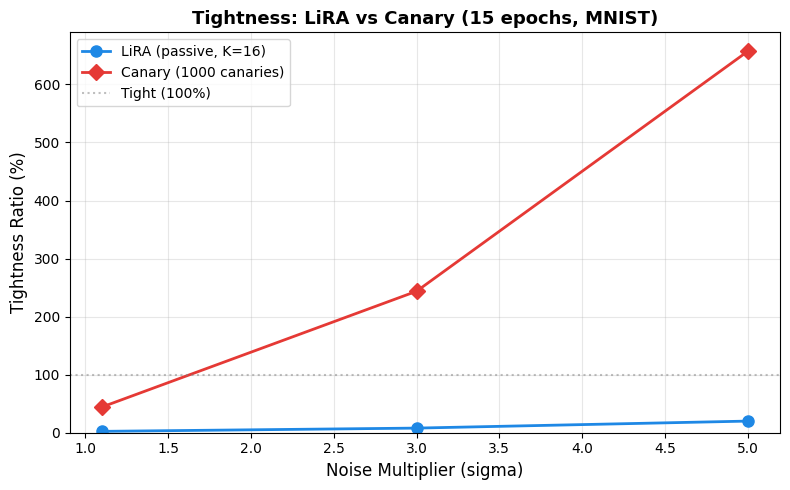
\includegraphics[width=0.92\linewidth]{figures/canary_vs_lira_tightness.png}
    \caption{Threat-model comparison from the 15-epoch MNIST validation run. Canary stress testing recovers substantially more leakage than passive LiRA at $\sigma=1.1$, matching the expected ordering between evaluator-controlled and final-model-only auditors.}
    \label{fig:canary_vs_lira}
\end{figure}

The strongest clean result from the extended MNIST canary rerun occurs at $\sigma=1.1$: with 1000 canaries and 5 audit seeds, the canary track reaches about 44.3\% tightness, while passive LiRA at the same setting remains much weaker. This validates the framework's threat-model separation: the stronger evaluator-controlled track produces stronger leakage evidence, while the passive track remains conservative under the same model family.

\begin{figure}[h]
    \centering
    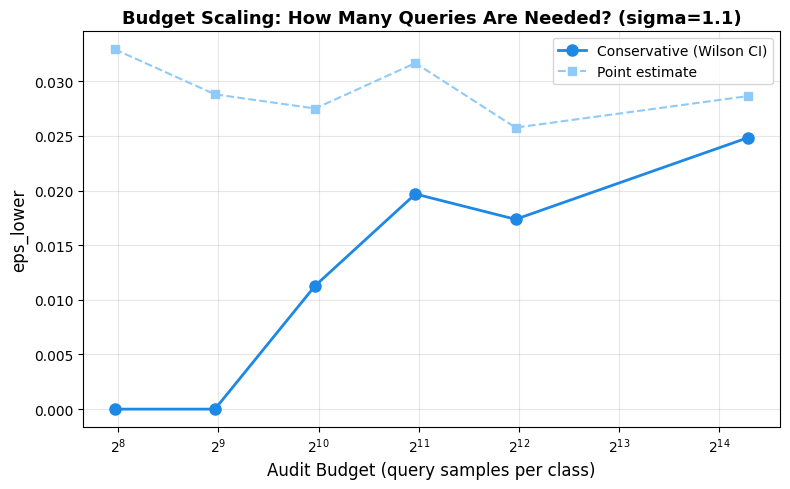
\includegraphics[width=0.92\linewidth]{figures/budget_scaling.png}
    \caption{Budget scaling for point estimates versus Wilson-supported conservative estimates. The gap between the optimistic and conservative curves shows why the framework reports confidence-supported lower bounds rather than sparse-tail point estimates.}
    \label{fig:budget_scaling}
\end{figure}

The budget-scaling experiment explains why small audit budgets are dangerous. Point estimates can look strong at low support, but Wilson-supported conservative estimates require enough member and non-member samples before reporting positive leakage. This behavior is central to the framework contribution: the pipeline is designed to reject attractive but statistically unsupported numbers.

\begin{figure}[h]
    \centering
    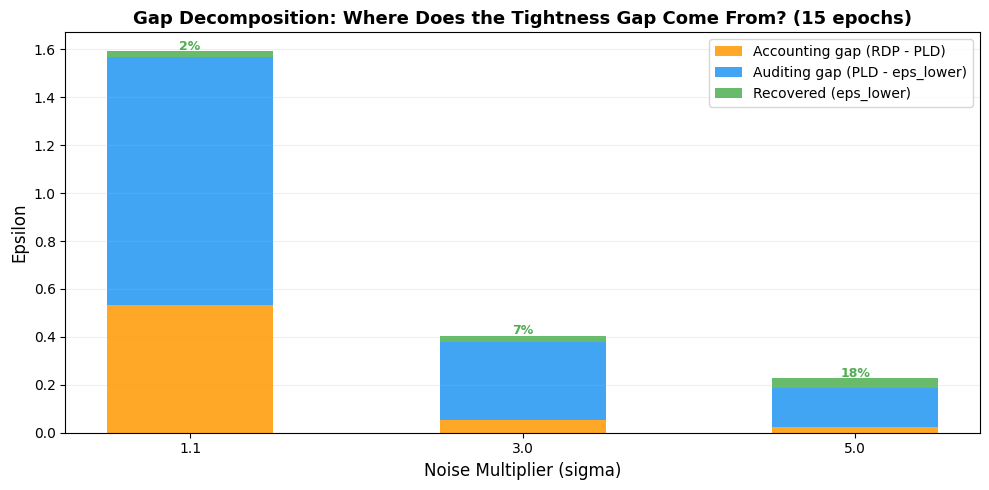
\includegraphics[width=0.92\linewidth]{figures/gap_decomposition.png}
    \caption{Gap decomposition from the sigma sweep. The framework separates recovered leakage, auditor gap, and accounting gap, making it possible to distinguish weak attacks from loose theoretical accounting.}
    \label{fig:gap_decomposition}
\end{figure}

The gap-decomposition view is a central output of the framework. It shows that the tightness gap should not be interpreted as one monolithic failure. Part of the gap comes from the accountant, part from the auditor, and part from the selected threat model. This is why the project is framed as a measurement framework: its purpose is to organize those sources of looseness cleanly enough that future stronger attacks can be compared fairly.

\section{Framework Validation}

The central claim of this project is that the implementation is a useful framework for auditing DP-SGD tightness, not that the current attacks close the gap. We validated the framework along four axes.

\textbf{Threat-model separation.} Canary stress testing and passive auditing are implemented as separate experiment tracks with separate configurations, outputs, and interpretation. This matters because canary insertion is an evaluator-controlled stress test, while passive auditing is a post-deployment model-only setting. The framework does not mix their scores or treat their bounds as interchangeable.

\textbf{Reproducibility and artifact integrity.} Runs save model artifacts, configuration snapshots, audit outputs, and JSON summaries. Result records are schema-validated before downstream aggregation, which prevents missing-key or malformed-result errors from silently entering the analysis. Seed propagation is explicit after the issue described in Section~\ref{sec:validity}; this makes repeated runs meaningfully seed-dependent rather than accidentally deterministic.

\textbf{Statistical conservatism.} The empirical lower-bound estimator reports both optimistic point estimates and confidence-supported conservative estimates. When the best threshold is supported only by a sparse tail, the framework flags the condition and reports the Wilson-supported value. This design choice intentionally lowers some impressive-looking numbers to zero when the sample size cannot justify a positive leakage claim.

\textbf{Sanity checks against the privacy contract.} A lower bound above $\varepsilon_{\text{upper}}$ is not treated as a discovery by default. It is treated as a diagnostic failure. Audit records now include an explicit validity flag indicating whether the reported empirical lower bound is at most the theoretical upper bound. The GDP diagnostic illustrates why this matters: in a small MNIST Raw LiRA comparison with 2048 training examples, 512 queries per audit seed, and $K \in \{8,16,32\}$ shadow models, Wilson estimates stayed below the PLD upper bound, while GDP estimates reached $1.86\times$ to $2.68\times$ the upper bound. The framework therefore marks GDP values that exceed the theoretical bound as invalid lower bounds and keeps them only as diagnostics. This behavior preserves useful diagnostic signals without turning failed estimator assumptions into privacy claims.

\section{Validity Checks and Limitations}
\label{sec:validity}

The validation process surfaced several implementation and statistical issues that affect how the results should be interpreted. We document them because they are central to the framework's reliability checks.

\textbf{Seed propagation.} The identical canary results across all three training seeds (Table~\ref{tab:canary}) stemmed from the experiment seed not being passed through to the canary generation and audit phases, so every run used the same effective random state. After fixing seed propagation, the three seeds produce meaningfully different $\varepsilon_{\text{lower}}$ values (standard deviation 0.668), confirming that the pipeline now responds to seed variation as expected.

\textbf{Pathological bounds.} After the seed fix, several runs---both canary and passive---produced $\varepsilon_{\text{lower}} > \varepsilon_{\text{upper}}$, with ratios as high as $2.3\times$. This happens when the threshold sweep lands on a sparse tail of the score distribution and small-sample noise inflates the TPR/FPR ratio. It is a known issue in auditing with limited samples~\citep{nasr2023tight}. We addressed this by adding confidence-aware reporting: when the selected threshold lies in a sparse region, we report the conservative Wilson-interval-based bound instead of the point estimate. Under this stricter mode, the canary bounds drop to $\varepsilon_{\text{lower}} = 0.0$, meaning the confidence intervals cannot support a positive leakage claim at the current sample size. This tells us we need more samples to make a positive leakage claim, not that leakage is absent.

\textbf{Score direction in passive auditing.} The initial passive pipeline did not properly align score direction across all scoring rules. For example, negative loss should decrease (become more negative) for non-members, but without explicit alignment the threshold sweep could select non-member-favoring events, producing inflated or meaningless bounds. The correction enforces consistent member-favoring constraints and proper direction mapping, which reduced the mean passive $\varepsilon_{\text{lower}}$ by roughly 95\% for the probability-margin score rule and eliminated many---though not all---pathological cases. The remaining pathological entries (Table~\ref{tab:passive}) reflect the fundamental difficulty of separating member and non-member distributions with small query budgets.

\textbf{Unmatched canary design.} In extended runs at high noise ($\sigma \in \{3.0, 5.0\}$), the canary track produced $\varepsilon_{\text{lower}}$ values exceeding $\varepsilon_{\text{upper}}$ by up to $6.6\times$. The cause is a design asymmetry: inserted and reference canaries were structurally different images (different patch positions and intensities), so the auditor could separate them by \emph{appearance} rather than by membership. This is a concrete, evaluator-controlled instance of the distribution-shift confound recently formalized for observational audits by Cebere et al.~\citep{cebere2026zerorun}, and a violation of the exchangeable-inclusion assumption underlying one-run auditing~\citep{steinke2023privacy}. Since $\varepsilon_{\text{lower}} > \varepsilon_{\text{upper}}$ is the field's standard signal of a real privacy bug~\citep{tramer2022debugging}, an audit pipeline that can raise this signal spuriously is dangerous; the fix is matched canary design, where inserted and reference canaries are exchangeable draws from a single pool.

\textbf{GDP estimator mismatch.} The GDP diagnostic was added to reduce dependence on threshold selection. It behaved sensibly on simple score-separation tests, but on Raw LiRA pilot runs it produced conservative estimates above the PLD upper bound. Rather than reporting those values as stronger lower bounds, the framework flags them as invalid for tightness reporting. This failure is useful: it shows that the framework can reject an estimator whose assumptions are inconsistent with the observed audit data.

\section{Reproducibility Artifacts}
\label{sec:reproducibility}

The framework is organized so that the reported numbers can be traced back to scripts and saved artifacts rather than manual spreadsheet edits. The core package lives under \texttt{src/dp\_audit\_tightness}. Experiment entry points live under \texttt{experiments/} for the general framework and under \texttt{codex/} for validation pilots. Generated validation artifacts are saved under \texttt{results/} and \texttt{codex/results/}.

The most important validation commands are:

\begin{itemize}
    \item \texttt{python -m unittest discover -s tests}, which checks lower-bound estimation, canary seed propagation, and GDP estimator behavior.
    \item \texttt{python experiments/run\_train.py --config configs/train/mnist\_mlp\_dp\_sgd.yaml}, which validates DP-SGD training and theoretical accounting.
    \item \texttt{python experiments/run\_audit\_canary.py --config configs/canary/random\_canary.yaml}, which validates evaluator-controlled canary auditing.
    \item \texttt{python experiments/run\_audit\_passive.py --config configs/passive/baseline\_passive.yaml}, which validates final-model-only passive auditing.
    \item \texttt{python experiments/correlate\_audit\_results.py --results-root results --output-dir results/comparisons}, which correlates training, canary, and passive artifacts while preferring valid lower-bound records over diagnostic pathologies.
    \item \texttt{python codex/run\_gdp\_comparison.py}, which compares Wilson and GDP-style lower-bound estimates and confirms that GDP is diagnostic-only in the Raw LiRA setting.
\end{itemize}

For final reporting, the trusted empirical privacy quantity is the Wilson-supported conservative $\varepsilon_{\text{lower}}$. Point estimates and GDP estimates are retained in artifacts because they are useful for diagnosis and model-fit analysis, but they are not used as validated lower bounds when they are sparse-tail dominated or exceed $\varepsilon_{\text{upper}}$. Future canary and passive audit records also store a \texttt{valid\_empirical\_lower\_bound} flag and a \texttt{sanity\_warning} field so downstream summaries can filter diagnostic failures cleanly.

\section{What Comes Next}

This report validates the framework and identifies which pieces are ready for scientific use. Several concrete next steps will move the project from framework validation toward stronger empirical conclusions:

\textbf{Stronger canary attacks.} Our current canaries are hand-designed pixel patterns. Gradient-based canary optimization, as used in~\citep{nasr2023tight, steinke2023privacy}, should substantially narrow the gap.

\textbf{Stronger passive attacks.} The current scoring rules are simple heuristics. Training a dedicated membership inference classifier or scaling likelihood-ratio methods~\citep{carlini2022membership} to more shadow models should produce tighter passive bounds.

\textbf{More data and bigger models.} MNIST with a 2-layer MLP and one epoch of training is a minimal setup. Moving to CIFAR-10 and deeper networks with longer training would produce more realistic leakage signals.

\textbf{Larger sample budgets.} The collapse of confidence-aware canary bounds to zero in small-sample corrected runs tells us we need more canaries and more repeated runs to make statistically grounded claims.

\textbf{Estimator validation.} GDP-style AUC estimation should remain diagnostic until it is calibrated on distributions where the implied lower bound is known to stay below the theoretical upper bound. Wilson confidence bounds remain the trusted reporting path for the current framework.

\textbf{Systematic saturation analysis.} With a wider range of auditor strengths, we can trace out the curve of $\varepsilon_{\text{lower}}$ vs.\ auditor strength and determine where saturation occurs.

\section{Conclusion}

We built and validated a framework for measuring the tightness gap between DP-SGD's theoretical privacy guarantees and what concrete auditing attacks can demonstrate. The framework supports two separated threat models, multiple auditor variants, RDP and PLD accounting, confidence-aware lower-bound estimation, artifact validation, and sanity checks that reject unsupported or contradictory estimates. On MNIST, the current attacks show the expected qualitative pattern: evaluator-controlled canaries demonstrate more leakage than passive final-model-only attacks, while conservative confidence bounds prevent sparse-tail artifacts from becoming privacy claims. The main contribution is therefore a reliable scaffold for future DP auditing experiments. With the framework validated, the next step is to scale the attacks, budgets, and datasets to determine how much of the remaining tightness gap comes from loose accounting and how much comes from weak auditors.

\bibliographystyle{plainnat}
\bibliography{references}

\end{document}
